\documentclass{standalone}
\usepackage{tikz}

\begin{document}

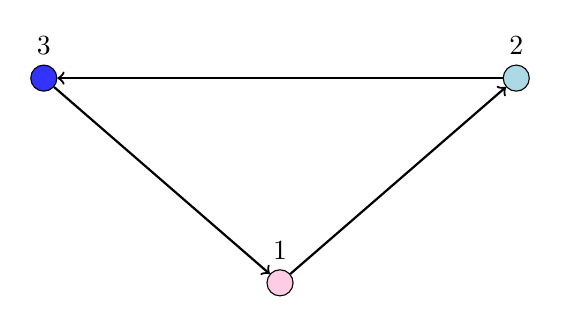
\begin{tikzpicture}[scale=2]
    % Define colors
    \definecolor{pinkish}{RGB}{255, 204, 229}
    \definecolor{bluish}{RGB}{173, 216, 230}
    
    % Nodes
    \node[circle, draw, fill=pinkish, label=above:1] (A) at (0,0) {};
    \node[circle, draw, fill=bluish, label=above:2] (B) at (1.5,1.3) {};
    \node[circle, draw, fill=blue!80, label=above:3] (C) at (-1.5,1.3) {};
    
    % Edges
    \draw[thick, ->] (A) -- (B);
    \draw[thick, ->] (B) -- (C);
    \draw[thick, ->] (C) -- (A);
\end{tikzpicture}

\end{document}